\chapter{Introducción}
\label{ch:introduccion}

El surgimiento de nuevas herramientas y tecnologías ha hecho posible mejorar las técnicas de ciberseguridad, tanto las técnicas para proteger la información, como las que explotan las brechas de seguridad. Este mismo desarrollo tecnológico hace que se incrementen de forma exponencial los ataques de \textit{malware}, es decir, cualquier tipo de \textit{software} diseñado para dañar, interrumpir, robar o acceder sin autorización a sistemas informáticos. La mejora de las técnicas de ciberseguridad ha provocado que los ciberdelincuentes se esfuercen aún más por conseguir su objetivo.

\vspace{1em}

En 1971, Creeper \cite{creeper}, el primer \textit{malware} de la historia, fue desarrollado por Bob Thomas Morris como un experimento y no causaba daño en los sistemas. Creeper era un gusano que se autorreplicaba y propagaba a través de ARPANET, y mostraba el mensaje <<\textit{I'm the creeper, catch me if you can!}>>. El primer \textit{malware} con impacto mundial, afectando a un 10\% de los 60000 servidores que había en ARPANET \cite{arpanet}, fue el gusano Morris \cite{morris}, desarrollado en 1988 por Robert Tappan Morris. Morris intentaba obtener la contraseña de los equipos en los que se ejecutaba mediante fuerza bruta, es decir, permutaba los nombres de usuarios conocidos y una lista de las contraseñas más comunes. Creeper y el gusano Morris provocaron la aparición de Reaper, el primer antivirus de la historia y la creación del Equipo de Respuesta ante Emergencias Informáticas (CERT, del inglés \textit{Computer Emergency Response Team}) \cite{cert}.

\vspace{1em}

Uno de los casos recientes más sonados fue WannaCry \cite{wannacry} en 2018, \textit{ransomware} \cite{ransomware} que bloquea el acceso a partes del sistema y pide un rescate. Este \textit{malware} causó un gran impacto a nivel mundial, afectando en España a empresas como Telefónica o Iberdrola \cite{noticia_wannacry}.

\vspace{1em}

Este aumento en la complejidad de las técnicas usadas tanto para dañar los sistemas como para evitar su detección, ha hecho que los métodos tradicionales basados en firmas \cite{firmas} para detectar patrones únicos en el código queden obsoletos. A día de hoy se combina con la heurística y sigue siendo una de las técnicas más usadas, pero son insuficientes para enfrentar vectores desconocidos.


\vspace{1em}

En los últimos años, uno de los campos más estudiados en  informática y con mayor avance y previsión de futuro es el aprendizaje automático \cite{ml}. Este es un campo de estudio dentro de la inteligencia artificial que se centra en aprender patrones a partir de datos, en lugar de seguir reglas programadas explícitamente. El sistema entrena con ejemplos y luego generaliza para hacer predicciones o tomar decisiones. El aprendizaje automático podría ser una solución eficiente y escalable para la detección y clasificación de \textit{malware}.

\vspace{1em}

A lo largo de este proyecto se tratará de evaluar la efectividad de diferentes modelos de aprendizaje automático para identificar este tipo de programas. Para ello tendremos en cuenta precisión, velocidad y capacidad de adaptación ante nuevas variantes de amenazas tratando de identificar las ventajas y limitaciones de cada método.

\vspace{1em}

Según Purplesec, con datos recogidos hasta 2018, el \textit{malware} sigue siendo uno de los ataques más usados y estima que se crean aproximadamente 230000 muestras nuevas cada día. Además cree que cada ataque con \textit{malware} cuesta de media unos 2,5 millones de dólares a las compañías. En la Figura \ref{fig:infeccxyear} podemos ver como ha evolucionado el número de infecciones por año \cite{purplesec}.

\begin{figure}[H]
	\centering
	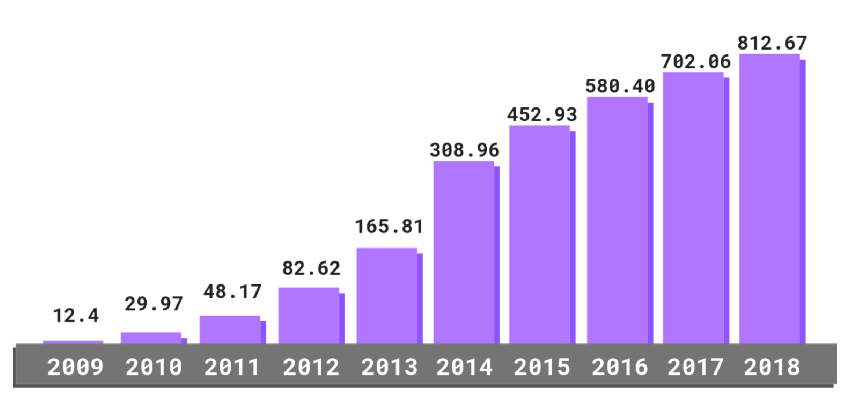
\includegraphics[width=1\textwidth]{Imagenes/incremento_malware}
	\caption{Millones de infecciones por año}
	\label{fig:infeccxyear}
\end{figure}
